% Autor: Leonhard Segger, Alexander Neuwirth
% Datum: 2017-10-30
\documentclass[
	% Papierformat
	a4paper,
	% Schriftgröße (beliebige Größen mit „fontsize=Xpt“)
	12pt,
	% Schreibt die Papiergröße korrekt ins Ausgabedokument
	pagesize,
	% Sprache für z.B. Babel
	ngerman
]{scrartcl}

% Achtung: Die Reihenfolge der Pakete kann (leider) wichtig sein!
% Insbesondere sollten (so wie hier) babel, fontenc und inputenc (in dieser
% Reihenfolge) als Erstes und hyperref und cleveref (Reihenfolge auch hier
% beachten) als Letztes geladen werden!

% Silbentrennung etc.; Sprache wird durch Option bei \documentclass festgelegt
\usepackage{babel}
% Verwendung der Zeichentabelle T1 (Sonderzeichen etc.)
\usepackage[T1]{fontenc}
% Legt die Zeichenkodierung der Eingabedatei fest, z.B. UTF-8
\usepackage[utf8]{inputenc}
% Schriftart
\usepackage{lmodern}
% Zusätzliche Sonderzeichen
\usepackage{textcomp}

% Mathepaket (intlimits: Grenzen über/unter Integralzeichen)
\usepackage[intlimits]{amsmath}
% Ermöglicht die Nutzung von \SI{Zahl}{Einheit} u.a.
\usepackage{siunitx}
% Zum flexiblen Einbinden von Grafiken (\includegraphics)
\usepackage{graphicx}
% Abbildungen im Fließtext
\usepackage{wrapfig}
% Abbildungen nebeneinander (subfigure, subtable)
\usepackage{subcaption}
% Funktionen für Anführungszeichen
\usepackage{csquotes}
% Zitieren, Bibliographie
\usepackage{biblatex}


% Zur Darstellung von Webadressen
\usepackage{url}
%chemische Formeln
\usepackage[version=4]{mhchem}
% siunitx: Deutsche Ausgabe, Messfehler getrennt mit ± ausgeben
\usepackage{floatrow}
\floatsetup[table]{capposition=top}
% Verlinkt Textstellen im PDF-Dokument
\usepackage[unicode]{hyperref}
% "Schlaue" Referenzen (nach hyperref laden!)
\usepackage{cleveref}
\sisetup{
	locale=DE,
	separate-uncertainty
}
%\bibliography{6Mi_M3_29-11-2017_References}

\begin{document}
	
	\begin{titlepage}
		\centering
		{\scshape\LARGE Versuchsbericht zu \par}
		\vspace{1cm}
		{\scshape\huge M4 - Stoßgesetze\par}
		\vspace{2.5cm}
		{\LARGE Gruppe 6Mi \par}
		\vspace{0.5cm}
		
		{\large Alexander Neuwirth (E-Mail: a\_neuw01@wwu.de) \par}
		{\large Leonhard Segger (E-Mail: l\_segg03@uni-muenster.de) \par}
		\vfill
		
		durchgeführt am 06.12.2017\par
		betreut von\par
		{\large Semir Vrana}
		
		\vfill
		
		{\large \today\par}
	\end{titlepage}
	\tableofcontents
	\newpage
	
	\section{Kurzfassung}
	Um vollständig elastische Stoßprozesse durchzuführen, wurden zwei Versuche durchgeführt.
	Diese waren so konzipiert, dass sie Rückschlüsse auf den Zusammenhang zwischen den Massen und Geschwindigkeiten vor und nach einem zentralen, elastischen und geraden Stoß zulassen. 
	Im ersten Versuch wurde dies durch zwei Fadenpendel mit daran hängenden Kugeln verwirklicht.
	Dabei wurde die resultierende horizontale Auslenkung der gestoßenen Kugel in Abhängigkeit von der initialen Auslenkung der stoßenden erfasst.
	Hier war zu erwarten, dass das Massenverhältnis der Kugeln, das mit diesem Versuch ermittelt wurde, gleich (bzw. fehlerüberschneidend) mit dem, das durch Wiegen ermittelt wurde, ist.
	Diese Überschneidung konnte tatsächlich festgestellt werden.
	Im zweiten Versuch wurde der Stoß durch eine Kugel, die eine Fallrinne hinunterrollt und dann auf eine Kugel am Fadenpendel trifft, untersucht.
	Dabei wurde der für den Stoß nutzbare Anteil der Höhenenergie der rollenden Kugel ermittelt und mit dem durch die Theorie erwarteten Wert verglichen.
	Die Unsicherheit des experimentell bestimmten Anteils beinhaltete den theoretischen Wert nicht, jedoch war die relative Abweichung zu klein, um die Theorie anzweifeln zu müssen.
	
	\section{Methoden}
	\subsection{Bestimmung der Massen}
	Die Massen der drei verwendeten Kugeln wurden mithilfe einer Waage gemessen.
	Dazu wurde zunächst die Waage mit aufgelegtem Ring auf Null gesetzt und dann abwechselnd die Kugeln in den Ring gelegt und die Anzeige der Waage abgelesen.
	Der Ring hatte den Zweck, die Kugeln nicht von der Waage rollen zu lassen.
	
	\subsection{Stoß zweier Pendelkugeln} 
	Zwei Kugeln unterschiedlicher Masse wurden mit Seilen hintereinander aufgehängt, sodass sie zwei Fadenpendel bildeten, und die Seile so justiert, dass die Schwerpunkte der Kugeln sich in der Ruhelage auf einer Höhe und in der Pendelebene befanden.
	Die Seile waren dabei jeweils an beiden Enden an einem Träger befestigt.
	Mit einem Maßband wurde die Pendellänge gemessen.
	Dann wurde für beide Pendelkugeln nacheinander folgende Messung durchgeführt:
	Die Pendelkugel wurde ausgelenkt und mithilfe von verschiebbaren Markierungen auf einer Maßschiene die Auslenkung festgestellt.
	Dann wurde die Kugel losgelassen und mit einer zweiten Markierung, die nach menschlichem Ermessen so platziert wurde, dass die gestoßene Kugel sie bei ihrer Schwingung gerade nicht berührte, die resultierende Auslenkung der zweiten Kugel bestimmt.
	Diese Messung wurde für fünf verschiedene Auslenkungen je fünf mal durchgeführt, um über diese Messungen mitteln zu können.
	\subsection{Stoß einer Kugel auf der Fallrinne mit einer Pendelkugel}
	Eine leichtere Kugel wurde eine Fallrinne herunter rollen gelassen und die Auslenkung einer Pendelkugel, die von ersterer angestoßen wurde, in gleicher Art und Weise wie zuvor gemessen.
	Diese Messung wurde für sechs verschiedene Starthöhen der kleinen Kugel auf der Fallrinne ebenfalls je fünf mal durchgeführt.
	Gemessen wurde hierbei der Abstand zum oberen Ende der Fallrinne.
	Um daraus die Starthöhe der Kugel bestimmen zu können, wurde die Fallrinne mit einer Messlatte vermessen.
	
	
	\section{Ergebnisse und Diskussion}
	

	\subsection{Beobachtung}

	\subsubsection{Stoß zweier Pendelkugeln}
	In \cref{GraphKKaufGK} und \cref{GraphGKaufKK} sind die Mittelwerte der Auslenkung der gestoßenen Kugel gegen die Startauslenkung der stoßenden Kugel aufgetragen.
	Der lineare Zusammenhang ist beim Betrachten der Werte bereits erkennbar und außerdem sollte dieser auch der Theorie zufolge auftreten (\cref{StossGleichung}).
	Deshalb haben wir einen Fit mit dem \enquote{Scaled Levenberg-Marquardt}-Algorithmus, welcher die Methode der kleinsten Quadrate verwendet, durchgeführt.
	Für den Fit wurde die folgende Funktion zugrunde gelegt:
	
	\begin{equation}
		f(x)=a*x+b
	\end{equation}
	
	\begin{equation}
		\label{StossGleichung}
		a_2' = a_1 \frac{2m_1}{m_1+m_2} = a_1 m(a_2')
	\end{equation}
	Wenn man die Steigungen der Auslenkungen $a_2'$ und $a_1'$ addiert erhält man:
	\begin{equation}
		m(a_2') + m(a_1') = \frac{2m_1}{m_1+m_2} + \frac{2m_2}{m_2+m_1} = 2
	\end{equation}
	Die Summe der Steigungen (\cref{TabelleFits}) der linearen Fit-Funktionen beträgt \SI{1,87}{}.
	\begin{table}[tb]
	\centering
	\begin{tabular}{ l | c | c  }
		& Kleine stößt Große $a_1$ & Große stößt Kleine $a_2$ \\ \hline 
		m &  $\SI{0,5038 \pm 0,0147}{}$ &$\SI{1,3744 \pm 0,0203}{}$  \\
	\end{tabular}
	\caption{Steigungen die sich aus dem Fit ergeben.}
	\label{TabelleFits}
	\end{table}
	Aus den Steigungen lässt sich das Verhältnis der Massen bestimmen.
	\begin{equation}
		k = \frac{m(a_2')}{m(a_1')} = \frac{2m_1}{m_1+m_2} \frac{m_1+m_2}{2m_2} = \frac{m_1}{m_2} \\
	\end{equation}
	Mit \cref{Partielle_Unsicherheiten} lässt sich $u(k)$ wie in \cref{UnsicherheitGleichung} berechnen.
	\begin{equation}
	u(y) = \sqrt{  \sum_{i=0}^{N} \left( \frac{\partial f}{\partial x_i}u(x_i)\right)^2  }
	\label{Partielle_Unsicherheiten}
	\end{equation}
	\begin{equation}
		u(k) =  k \sqrt{\left(\frac{u(m(a_1'))}{m(a_1')}\right)^2 + \left(\frac{u(m(a_2'))}{m(a_2')}\right)^2 }
		\label{UnsicherheitGleichung}
	\end{equation}
	Es ergibt sich eine Massenverhältnis von $k_s$ =  \SI{2,7281 \pm 0,1068}{}. Die berechnete Unsicherheit wurde mit einem Faktor von \num{1,2} multipliziert gemäß der Studentschen $t$-Verteilung, da aus nur fünf Messpunkten eine Steigung ermittelt wurde.
	
	In \cref{MessungGewichte} sind die durch Wiegen festgestellten Massen der Kugeln aufgeführt. 
	Die Unsicherheit der Waage ist auf ihr als $u_\text{Waage}=0,01 \frac{m_\text{Messung}}{2\sqrt{3}} $ angegeben. Zusätzlich dazu zeigt die Digitalanzeige nur zwei Nachkommastellen an (also Typ B Unsicherheit mit rechteckiger WDF), woraus folgt: 
	\begin{gather*}
		u_\text{digital}=\frac{0,01 \si{g}}{2\sqrt{3}} \approx \SI{0,029}{g} \\
		\implies u_{\Delta m} = \sqrt{u_\text{Waage}^2 + u_\text{digital}^2}
	\end{gather*}
	Das Massenverhältnis durch Wiegen ergibt sich damit als $k_m$ = $\SI{2,6562 \pm 0,0109}{}$, wobei die Unsicherheit analog zu \cref{UnsicherheitGleichung} berechnet wurde. 
	\begin{table}[tb]
	\centering
	\begin{tabular}{ l | c | c  }
		& Große Kugel & kleine Kugel \\ \hline 
		Masse &$\SI{510,68 \pm 1,47}{g}$ &  $\SI{192,26 \pm 0,56}{g}$  \\ 
	\end{tabular}
	\caption{Massen, die sich beim Wiegen der Kugel ergeben.}
	\label{MessungGewichte}
	\end{table}
	


	\begin{figure}[htb]
	  \centering
	    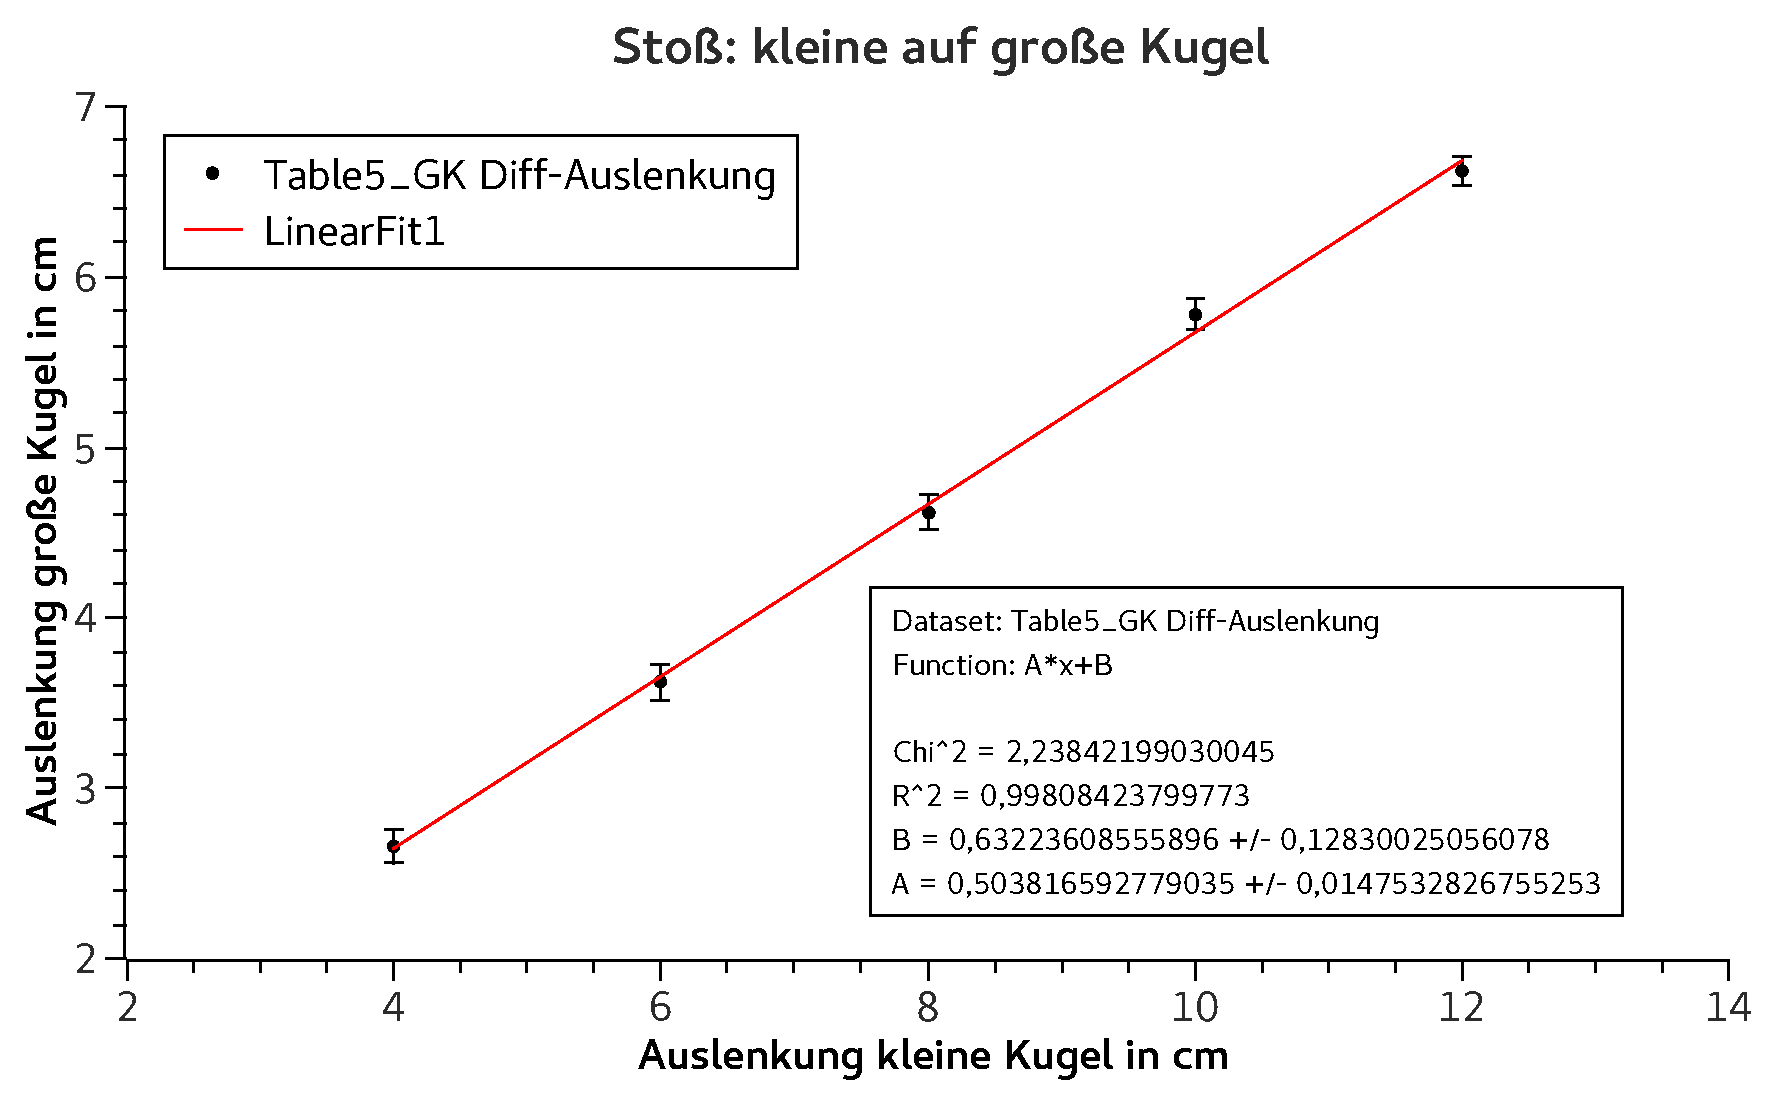
\includegraphics[width=1.0\textwidth]{StossKKaufGK}
	  \caption{Kleine Kugel stößt die große Kugel. Der x-Fehler ist kleiner als die Symbolgröße.}
		\label{GraphKKaufGK}
	\end{figure}
		
	\begin{figure}[htb]
	  \centering
	    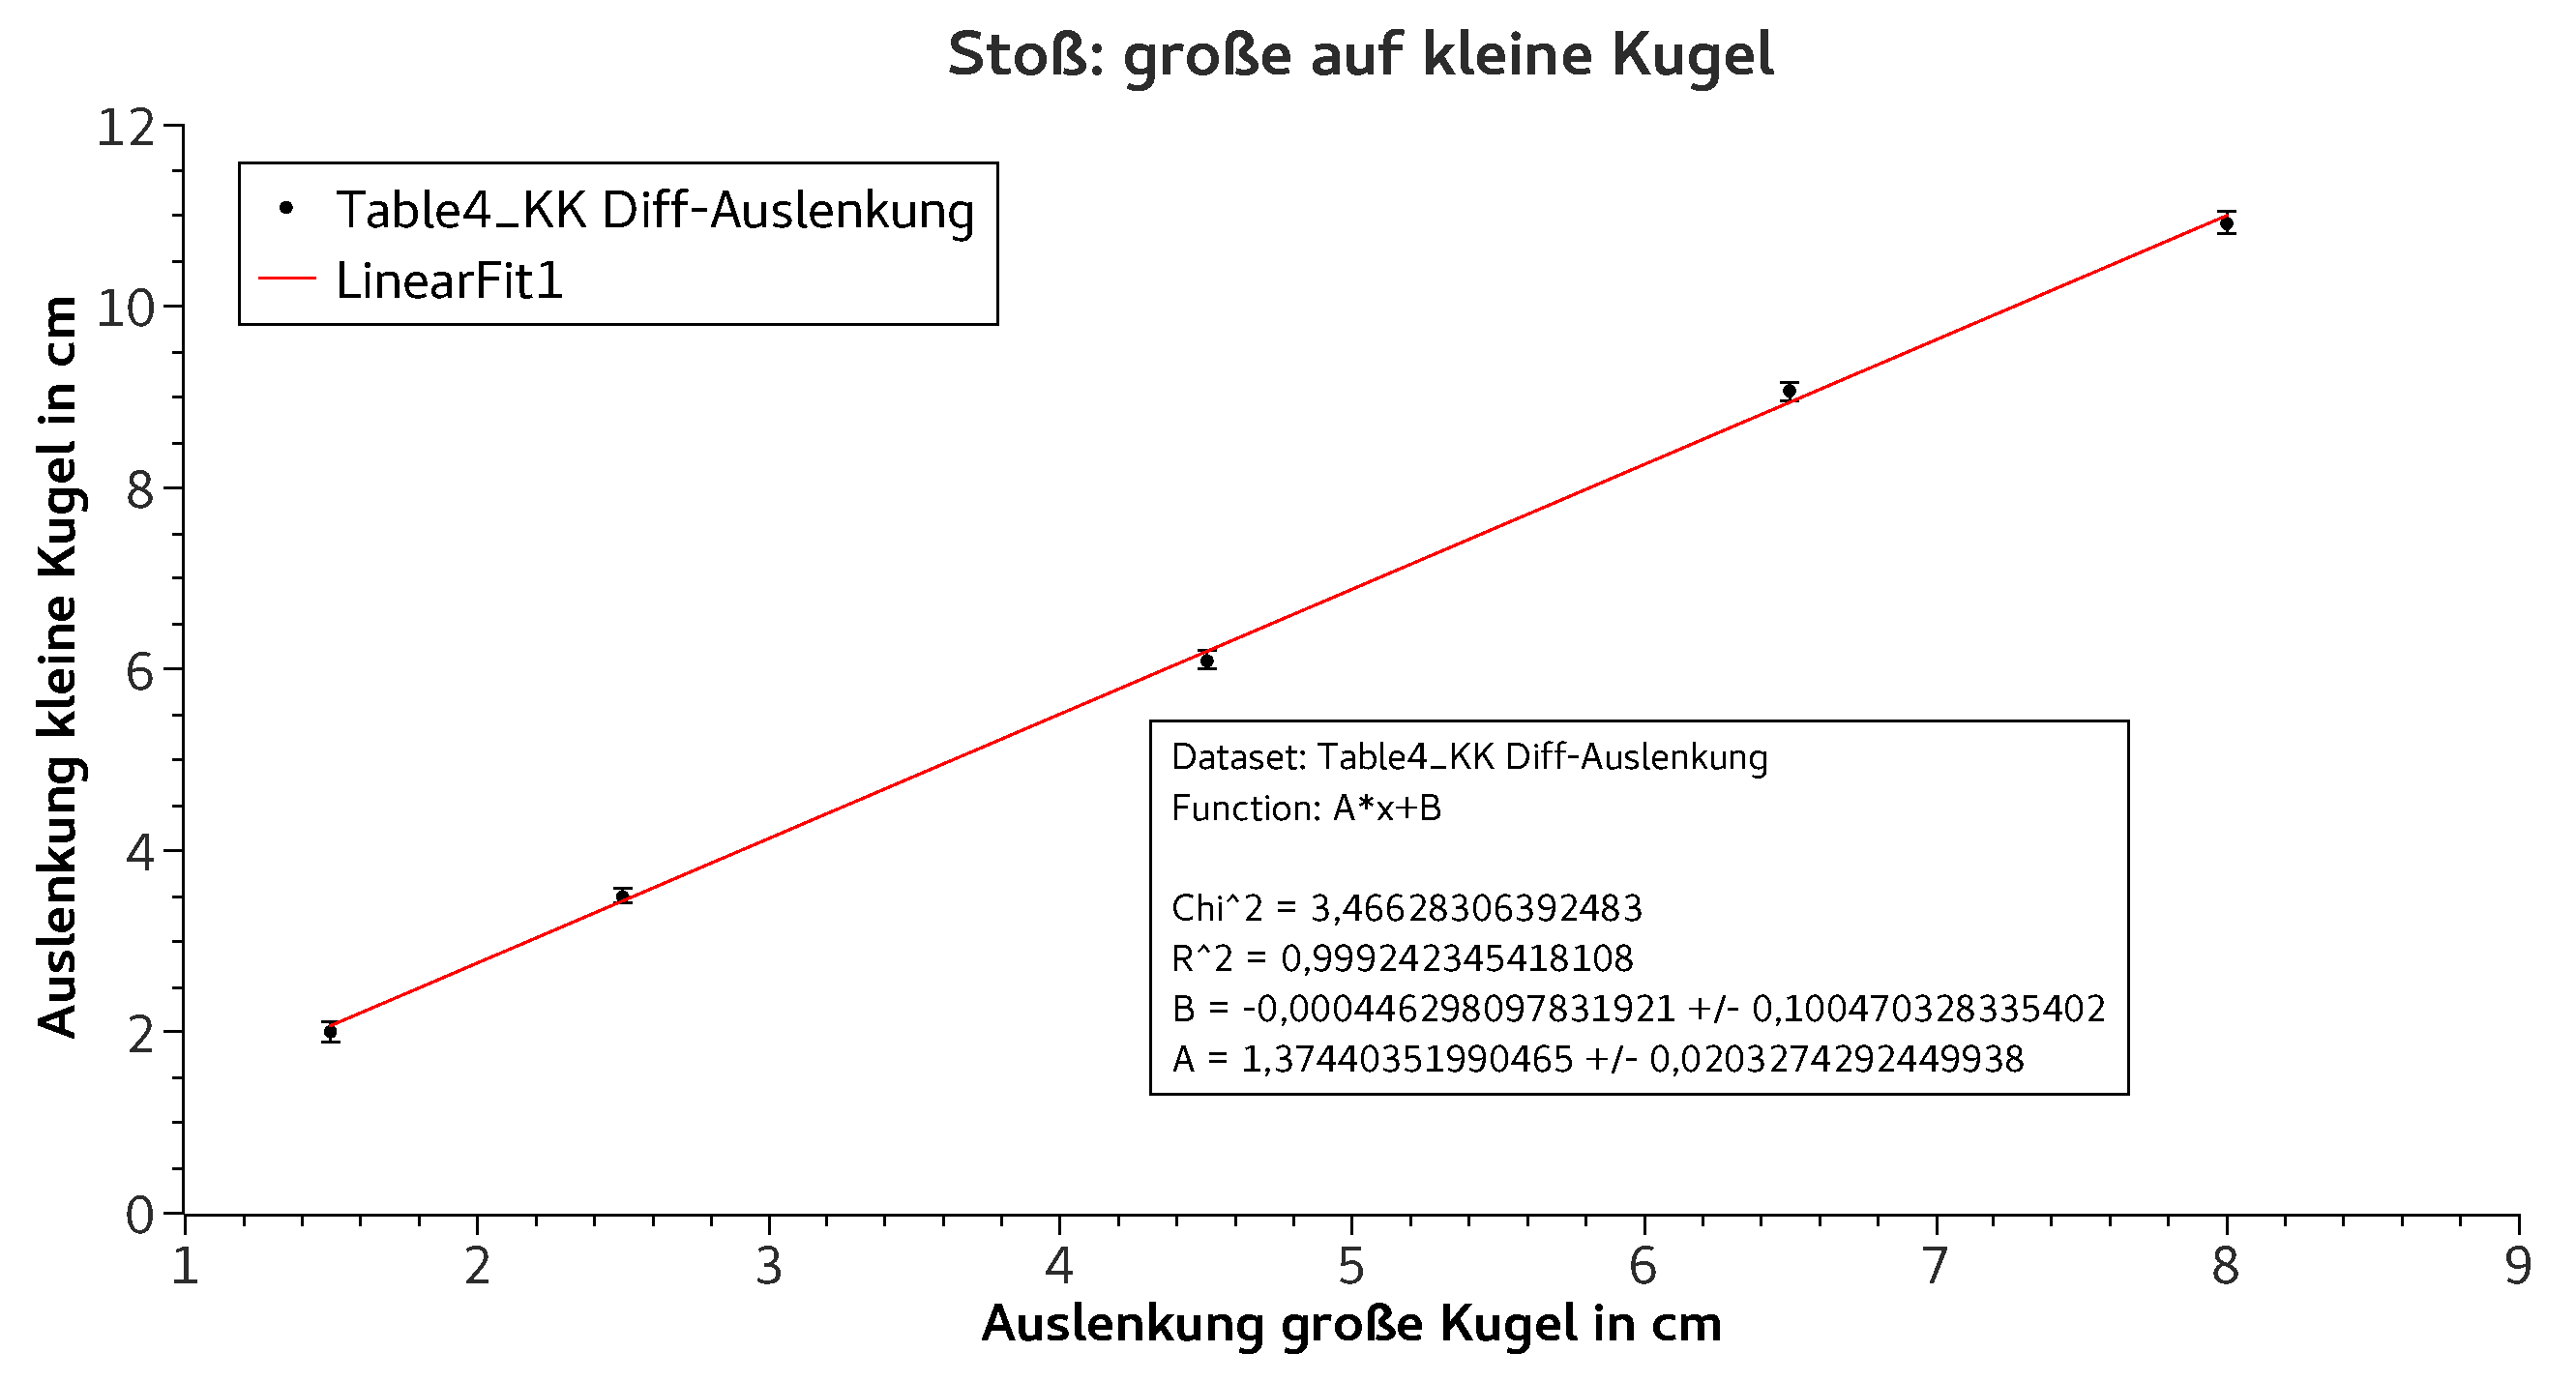
\includegraphics[width=1.0\textwidth]{StossGKaufKK}
	  \caption{Große Kugel stößt die kleine Kugel. Der x-Fehler ist kleiner als die Symbolgröße.}
		\label{GraphGKaufKK}
	\end{figure}


	\subsubsection{Stoß einer Kugel auf der Fallrinne mit einer Pendelkugel}

	\begin{figure}[htb]
	  \centering
	    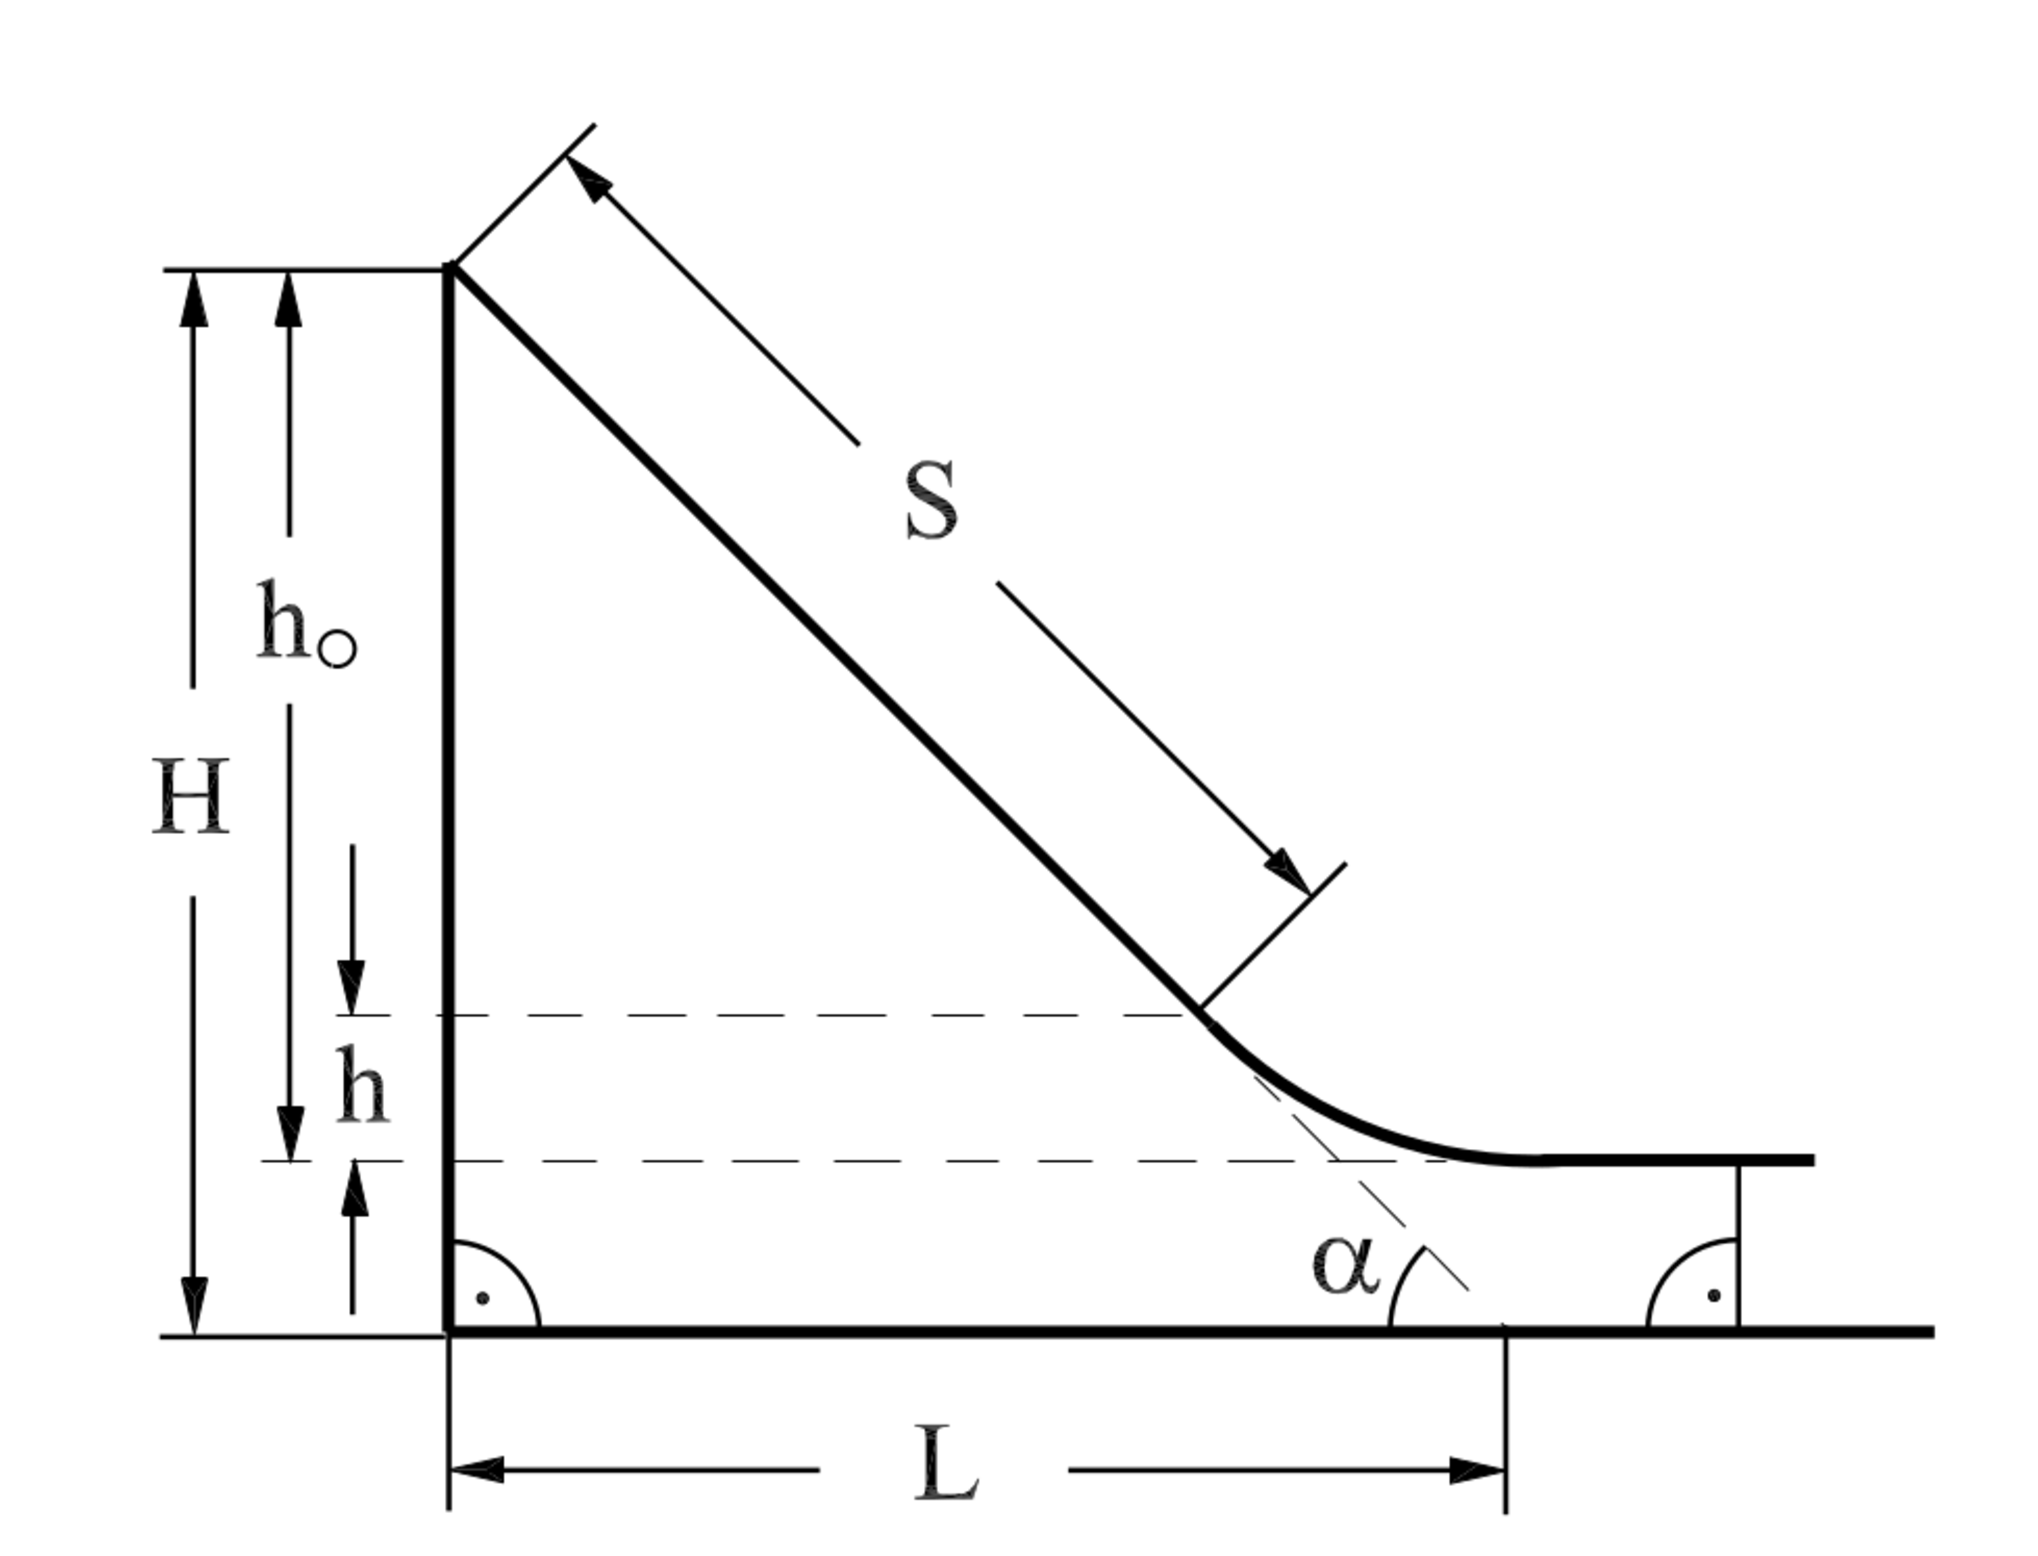
\includegraphics[width=0.5\textwidth]{Skizze}
	  \caption{Skizze der Fallrinne.}
	  \label{Skizze}
	\end{figure}


	Aus den Abmessungen $H$, $L$ und $h_0$ der Fallrinne (vgl. \cref{Skizze}) lässt sich die Fallhöhe wie folgt bestimmen:\\
	 Aus der Skizze ist ersichtlich, dass 
	\begin{equation}
		\sin(\alpha) s = h_0-h 
		\label{Sin1}
	\end{equation}
	und
	\begin{equation}
		\sin(\alpha) = \frac{H}{S} = \frac{H}{\sqrt{H^2+L^2}} = \frac{1}{\sqrt{1+L^2/H^2}}
		\label{Sin2}
	\end{equation}
	gilt. Fügt man \cref{Sin1} und \cref{Sin2} zusammen erhält man:
	\begin{equation}
		h = h_0 - \frac{s}{\sqrt{1+ L^2/H^2}}
		\label{GleichungFallhoehe}
	\end{equation}
	\begin{equation}
		u(h) = \sqrt{u(h_0)^2 + \frac{u(s)^2}{1+L^2/H^2} + s^2\frac{(u(L)LH)^2 + (u(H)L^2)^2}{(H^2 + L^2)^3} }
		\label{UnsicherheitFallhoehe}
	\end{equation}
	\begin{table}[tb]
	\centering
	\begin{tabular}{  l | c  }
		& Länge  \\ \hline 
		$H$ &  $\SI{0,328 \pm 0,00173}{m}$ \\ \hline 
		$h_0$ &  $\SI{0,317 \pm 0,00173}{m}$ \\ \hline 
		$L$ &  $\SI{0,535 \pm 0,00577}{m}$ 
	\end{tabular}
	\caption{Maße der Fallrinne.}
	\label{MessungFallrinne}
	\end{table}
	Aus \cref{GleichungFallhoehe} und \cref{MessungFallrinne} ergibt sich \cref{TabelleFallhoehe}. Setzt man in \cref{UnsicherheitFallhoehe} alle Werte außer $s$ und $u(s)$ folgt:
	\begin{equation}
		u(h) = \sqrt{ \SI{2,99e-6}+ 0,2732u(s)^2 + \SI{2,08e-5}s^2 }
	\end{equation}
	\begin{table}[tb]
	\centering
	\begin{tabular}{  c | c  }
		$s$  & $h$ \\ \hline 
		$\SI{0,00 \pm 0,0058}{m}$ &  $\SI{0,317 \pm 0,0035}{m}$ \\ \hline
		$\SI{0,10 \pm 0,0058}{m}$ &  $\SI{0,264 \pm 0,0035}{m}$ \\ \hline 
		$\SI{0,20 \pm 0,0058}{m}$ &  $\SI{0,212 \pm 0,0036}{m}$ \\ \hline
		$\SI{0,30 \pm 0,0058}{m}$ &  $\SI{0,160 \pm 0,0037}{m}$ \\ \hline
		$\SI{0,40 \pm 0,0058}{m}$ &  $\SI{0,101 \pm 0,0039}{m}$ \\ \hline 
		$\SI{0,50 \pm 0,0058}{m}$ &  $\SI{0,056 \pm 0,0042}{m}$  
	\end{tabular}
	\caption{Fallhöhe in Abhängigkeit von $s$.}
		\label{TabelleFallhoehe}
	\end{table}
	In \cref{GraphRKaufGK} ist die Wurzel der Fallhöhe gegen die Auslenkung der großen Kugel aufgetragen. 
	\begin{figure}[htb]
	  \centering
	    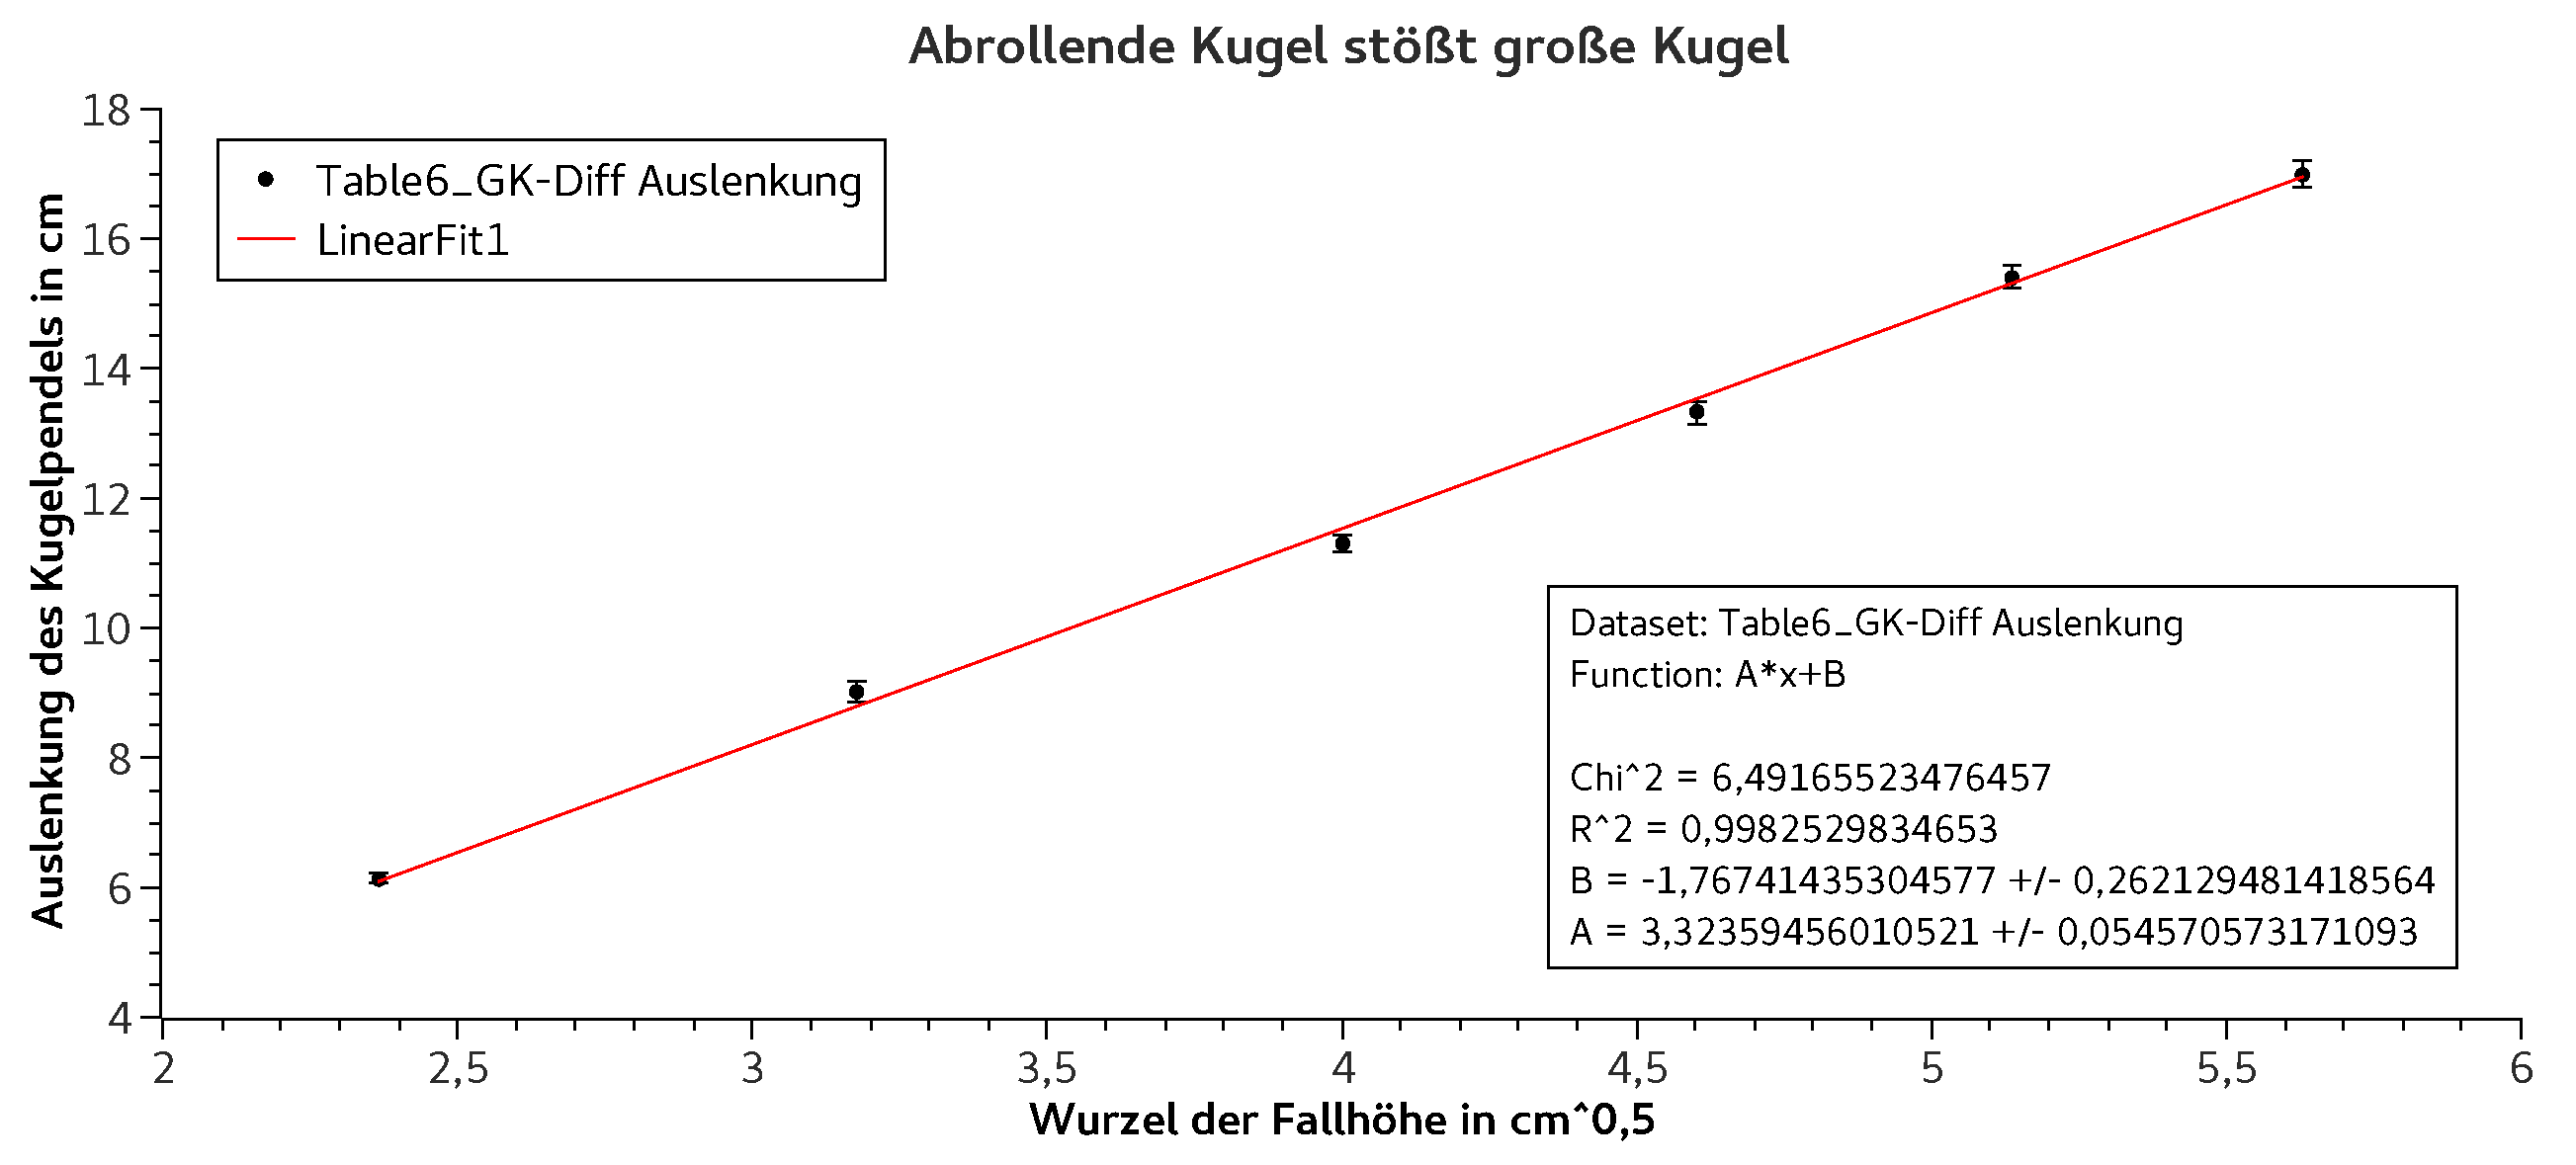
\includegraphics[width=1.0\textwidth]{StossRKaufGK} 
	  \caption{Die Kugel rollt die Fallrinne hinab und stößt die große Kugel. Der x-Fehler ist kleiner als die Symbolgröße.}
		\label{GraphRKaufGK}
	\end{figure}
	\cref{eGleichung} war in der Einführung zum Versuch vorgegeben.
	\begin{equation}
		\label{eGleichung}
		a_2' = \frac{2m_1}{m_1+m_2} \sqrt{\varepsilon} \sqrt{2 l} \sqrt{h}
	\end{equation}
	Aus dem linearen Fit kann man die Steigung $m(a)$ = $\SI{3,324 \pm 0,054}{\sqrt{cm}}$ ablesen. %find ich besser als cm^0,5
	Außerdem wurde die Länge des Pendels aufgenommen \SI{188,5 \pm 1,15}{cm} und die Masse der Kugel beträgt $m_1$ = \SI{63,70 \pm 0,18}{g}.
	Es folgt:
	\begin{equation}
		\varepsilon = \frac{(m_1+m_2)^2}{2(2m_1)^2l} m(a)^2 = \SI{0,596}{} 
	\end{equation}
	mit
	\begin{equation}
		u(\varepsilon) = \varepsilon\sqrt{ \left(\frac{2u(m(a))}{m(a)}\right)^2  + \left(\frac{u(l)}{l}\right)^2 + \left(\frac{u(m_1)2m_2}{m_1 (m_1+m_2)}\right)^2 + \left(\frac{2u(m_2)}{m_1+m_2}\right)^2} = \SI{0,020}{}
	\end{equation}


	\subsection{Diskussion}
	Wenn man beim Stoß zweier Fadenpendel das aus den Steigungen der Fit-Funktionen ermittelte Massenverhältnis ($k_s$ =  \SI{2,7281 \pm 0,1068}{}) mit dem durch Wiegen ermittelten Massenverhältnis ($k_m$ = $\SI{2,6562 \pm 0,0109}{}$) vergleicht, stellt man fest, dass sich die Intervalle der Unsicherheiten wie erwartet überschneiden.
	\par
	Beim Stoß einer Kugel auf der Fallrinne mit einer am Pendel aufgehängten Kugel wurde ein nutzbarer Energieanteil von $\varepsilon = \SI{0,596 \pm 0,02}{} $ ermittelt.
	Die Theorie gibt hierfür einen zu erwartenden Wert von $\varepsilon = \frac{\num{5}}{\num{9}} \approx \num{0,556}$ an, der nicht im Unsicherheitsintervall des experimentell ermittelten Wertes liegt, aber nur um die doppelte Unsicherheit abweicht.
	Als Grund für diese Abweichung könnte man zunächst Reibungsverluste an der Fallrinne vermuten, dies hätte aber einen geringeren experimentell ermittelten Wert als den Theorie-Wert zufolge, was nicht der Fall war.
	Demnach muss für die Abweichung eine Unsicherheit verantwortlich sein, die hier rechnerisch nicht erfasst werden konnte.
	Denkbar wäre hierbei die Art der Aufhängung in Form eines V-förmig gespannten Seils, bei der, um den zentralen Stoß zu justieren, sich nicht beide Enden auf der selben Höhe befanden und die zwischen den Messungen mitunter neu justiert werden musste, wenn die Kugel auf dem Seil verrutscht war.
	Des Weiteren wurde beim theoretischen Bestimmen des nutzbaren Energieanteils angenommen, dass die Kugel die Fallrinne ideal hinabrollt, jedoch kann die Kugel auch teilweise rutschen, was eine geringere Rotationsenergie zur Folge hätte und somit auch einen höheren nutzbaren Energieanteil verursachen würde.
	Außerdem war die Beschichtung der hängenden Kugel an einer Seite leicht demoliert und das Rückschwingen dieser Kugel nach dem Stoß verursachte einen Stoß gegen die Fallrinne, welcher deren Justierung beeinflusst haben kann.
	
	\section{Schlussfolgerung}
	Beim Stoß zweier Fadenpendel konnten wir die Theorie zum vollständig elastischen Stoß insofern experimentell bestätigen, als dass bei Bestimmung des Massenverhältnisses der Kugeln Werte mit überschneidenden Unsicherheitsintervallen ermittelt wurden, unabhängig davon, ob sie mit der Stoßtheorie oder durch einfaches Wiegen bestimmt wurden.
	Die Unsicherheiten waren hierbei ausreichend klein, um diesen Schluss zuzulassen, aber man könnte eine deutlich präzisere Messung durchführen, wenn man die Auslenkung der gestoßenen Kugel mit einem Ultraschallentfernungssensor statt mit der wenig genauen Messung mithilfe von verschiebbaren Markierungen erfasst hätte. \par
	Die Ermittlung des nutzbaren Energieanteils einer Kugel auf der Fallrinne ergab einen experimentell ermittelten Wert dessen Abweichung vom durch die Theorie vorausgesagten Wertes zwar nicht innerhalb der Messungenauigkeiten lag, aber nicht ausreichend deutlich abwich, um ein Infragestellen der Theorie zu rechtfertigen.
	Diese Abweichungen lassen sich durch äußere Einflüsse, die nicht durch Zahlenwerte ausgedrückt und somit nicht in die Unsicherheit miteinbezogen werden konnten, erklären.
	Präziser hätte man diese Untersuchungen durchführen können, wenn man beispielsweise mit einer Lichtschranke am waagerechten Teil der Fallrinne die Geschwindigkeit der Kugel gemessen hätte, um diese kinetische Energie mit der potentiellen Energie am Startpunkt der Bewegung zu vergleichen.
	%\printbibliography
\end{document}
